\chapter{Literature Review}
\label{literature_review}


As mentioned in the Introduction, it is only through the recent development of large open source datasets that statistical approaches to code related tasks have been available to machine learning researchers. 
As would be expected of any new and growing field, the range of attempted tasks is still expanding. 
Although as of writing no formal attempt has been made to translate fine grained elements of source code into their natural language descriptions, a great deal of relevant insight has been made in the related fields of source code summarization, variable naming, documentation generation, and code language modelling. Many of these problems highlight possible approaches to modelling the patterns and structure of code as language, and can even be cast into a machine translation framework.  

In this review we summarise the current advances of these methods and how they relate to the task at hand.  We start by examining with the general progress in the language modelling of code, before moving on to specific tasks that can be posed as sequence generation tasks, such code comment prediction, code summarization or function naming. We subsequently examine advance in the related fields of representation of programs, before we finally examine the existing datasets, and the scope of the problems they are suitable to address. 

\section{Language Models of Source Code}

The earliest work modelling source code with natural language techniques comes from Hindle at al \cite{hindle_naturalness_nodate}, who used simple Kneser-Ney smoothed n-gram models of code tokens, to create language models for large-scale Java and C projects.
With these models, Hindle was able to demonstrate that the cross-entropy of source code within projects was lower than that of large English corpora - indicating the presence of repetetive common patterns that could be leveraged for code completion, naming and summarization.
This was consistent with findings by Gabel and Su \cite{gabel_study_2010} who examined the lines of approximately 6000 projects of code and found widespread repetition of sections of up to several lines, both within and across projects.
Despite the simplistic Markov chain assumption implicit in the ngram model, the effectiveness of this modelling techniques, especially within projects, opened up the field of code analysis to the wider natural language processing community.

This model, which only took into the lexical structure of code, was subsequently improved by Nguyen et al\cite{nguyen_statistical_2013}, who by integrating semantic information into the n-gram model.
Instead of training on the raw string of the token, the \textit{lexeme}, this model condensed information such as data type, scope, role (such as literal, variable, function call) into a \textit{sememe}, and trained an n-gram topic model, modelling both local context \textit{sememes} ngrams, and global trends in the code.
This highlighted the value of taking into account the semantic information in code, as well as the lexical, in future prediction tasks.

Since then a number of different language models of code have formed, largely finding their use in code completion tasks. These are often most successful if they can take into account the long range dependencies of code, or elements of the code beyond simple lexical structure. For instance Tu et al added a cache mechanism to improve Hindle's ngram model in capturing long range dependencies  \cite{tu_localness_nodate}, while this itself was surpassed (up to 9 grams) with a basic recurrent neural model by White et al\cite{white_toward_2015}.
Most recently, Bhoopchand et al used a sparse pointer network to create a language model that significantly outperformed a LSTM baseline on code completion tasks, that was able to refer to objects in code over 60 tokens previous\cite{bhoopchand_learning_2016}.

This work in language modelling has direct applicability to our task at hand, as it points out relevant strategies in picking out the statistically important features of `natural' code. In particular we note the importance of capturing long range dependencies (as seen in neural models), with the performance benefit that can be brought by taking into account semantic information (from the instructions given to the computer).

\section{Sequence Generation from Code: Machine Pseudo-Translation}

Given the industrial importance of software engineers understanding sections of code, a long running task is that of code summarization. 
This task involves taking large sections of code blocks, and summarising its meaning in natural language. It has historically had parallels with the long running (inverse) problem of semantic parsing. CITE
As such, early approaches to this problem completely ignored the `naturalness' properties of code and its comments, and instead, automatic summarization of source code was tackled with rule-based methods. 

Work by Sridhara et al \cite{sridhara_[not_2010}  used static analysis to find important semantic subunits of code in Java projects, and used sets of sentence templates to produce English from these subunits.
% This model revolved around automatic rule-based summarization of the source code in the source code in consideration.
This work produced text that describe the functions in question to a high degree of accuracy, but Sridhara noted the potential lack of transferrability to other settings, and lack of examples with which to compare their summaries.  
This procedure was also inherently inflexible, relying on human crafted templates, and specified rules. Furthermore the size of the dataset, four projects in total, indicated a potential problem in the generalisability of the work to other domains, projects or even languages.

However, the advent of the statistical approaches to code language modelling led by Hindle et al \cite{hindle_naturalness_nodate} signalled the start of similar approaches to sequence generation. The earliest is Movshovitz-Attias et al \cite{movshovitz-attias_natural_nodate}, who used both ngrams and topic models such as LDA to predict comments from JAVA source code. In this they found that modelling the lexical components of source code as coming from a mixture of topics - "code" and "text" - outperformed models that ignored this distinction.  This pointed to the strength of taking into account features of code (such as distinguishing comments from commands), even if such destinction were still purely on the lexical level.

% Since then, statistical approaches have become more popular in attacking the problem, often involving much larger corpora of training data.
% Iyer et al \cite{iyer_summarizing_2016} sourced a large dataset of code snippets and questions from Stack Overflow, a popular programming website, to attempt this problem statistically.
Since then neural models have become popular methods of attacking sequence generation, as they capture long range dependencies in sequences, and have shown great promise in other neural translation tasks.

A particularly successful example is that of Iyer et al \cite{iyer_summarizing_2016}, who applied a neural attentional model to the problem of generate code summaries, training on a large collection of snippets and questions from the Stack Overflow.   

Their model combined two features: a distributed representation of the code, generated by attentional mechanism \cite{luong_effective_2015} over code token embeddings; and a Long Short Term Memory unit CITE to encoded natural language tokens. Together these generated descriptions as a sequence of conditional distributions, in an encoder-decoder model. 

Specifically this model calculated the probability of generating a length $l$
descriptive sequence through a product of conditional probabilities the previous $l-1$ tokens

$$P(\{n\}_1^l) = \prod_{i=1}^lp(n_i | n_1, ..., n_{i-1} ) $$

where each conditional probability was the proportional to a non-linear transformation of the combination of hidden state of the LSTM $\mathbf{h_i}$ and the attentional vector  $\mathbf{t_i}$ at that point in the sequence: 

$$\text p(n_i | n_1, ..., n_{i-1} ) \propto \mathbf{W}\text{tanh}(\mathbf{W_1h_i} + \mathbf{W_2t_i})$$

where $\mathbf{W} \in \mathbb{R}^{|N|\text{x} H}, \mathbf{W_1}$ and $\mathbf{W_2} \in \mathbb{R}^{H \text{x} H}$  and $ H$ is embedding dimensionality of words, $ N $ the vocabulary.\cite{iyer_summarizing_2016}
A visual schematic of the model is preseted in Figure \ref{fig:Iyer}.
Iyer et al then ran a beam search over the decoder to explore the space of likely sequences, and evaluated their generations using the BLEU-4 and METEOR metrics.

This model achieved a new record in the performance of the code summarization task, and outperformed rival NLP models such as MOSES, a traditional phrase-based machine translation model \textbf{CITE \& paraphrase}, and SUM-NN, another attention based summarization model using dense layers instead of LSTMs.CITE. It also achieved a first in learning to generate original sentences from arbitrary code sections, and has proved successful in other domains.  

Loyola et al \cite{loyola_neural_2017}, for instance, adapted a similar attention model to Iyers to generate short descriptions of differnces in code.
This time intead of training on a single piece of source code and questions, data was sourced to present pairs of code changes, `diffs', with comments describing the change, `commit messages'. 
In this setting, the attentional model was able to generate faesible messages, both within projects and between projects.

Both these attention models showed the effectiveness of being able to pickout relevant portions of code at different points in sequence generation, but failed to take into account the longer term correlations of the tokens in source code. In fact by only using this kind of attentional model to process source code, both models treat the source code as little more than bag of token embeddings.

In this regard, an improvement on these attentional models is that Alamanis et al \cite{allamanis_convolutional_2016}, which uses a convolutional attention network over tokens, for the task of predicting the names of functions given their body. 
%aiming to capture long range correlations in code through spatial convolutions instead of temporal hidden state.

In this model source code is split lexically in to a padded sequence of embedded tokens, over which a one dimensional convolution of fixed width is run, to create a number of attentional feature vectors $\mathbf{\{v_k\}}$.
These feature vectors are then point-wise multiplicatied with the hidden state of an rnn, $\mathbf{h_{t-1}}$, to be effectively `selected' for their relevance to next generated token, before being normalised.

This set of feature vectors is then convolved with an attention kernel, to give a set of attention weights, each corresponding to a token embedding. 
A final attention vector $\mathbf{\alpha}$ is constructed from the convex combination of the token embeddings under the attention weights, and this vector is used to generate a distribution over the next function subtoken.
An illustration of the algorithm with pseudo code is presented in Figure X.

The authors of this model apply it to both the narrow task of generatign function names, and that of code retrieval. In it they find that taking into account the long range features of the code in the convolutional model surpasses a baseline attentional model of the machine translation model originated by Bahdenau \cite{bahdanau_neural_2014}, and found that this performance was further improved by adding a cacheing mechanism to the model.

Both these attention models show the strengths that attention can provide in combining the modalities of text and code. However, a key failing of both models remains their lack of appreciation for the syntax and semantic of the underlying code.
Although Allamanis et al's model is more aware of the structure of lexical code tokens than Iyer et als, both models continue to ignore a fundamental channel of information communication through code - that of communication from human to computer.

\section{Representations of Code}



\section{Existing Datasets}

edinburgh
django
stack overflow


These attentional style models have shown great success at combining the different modalities of text and code, and this particular model
\begin{figure}[tb]
    \centering
    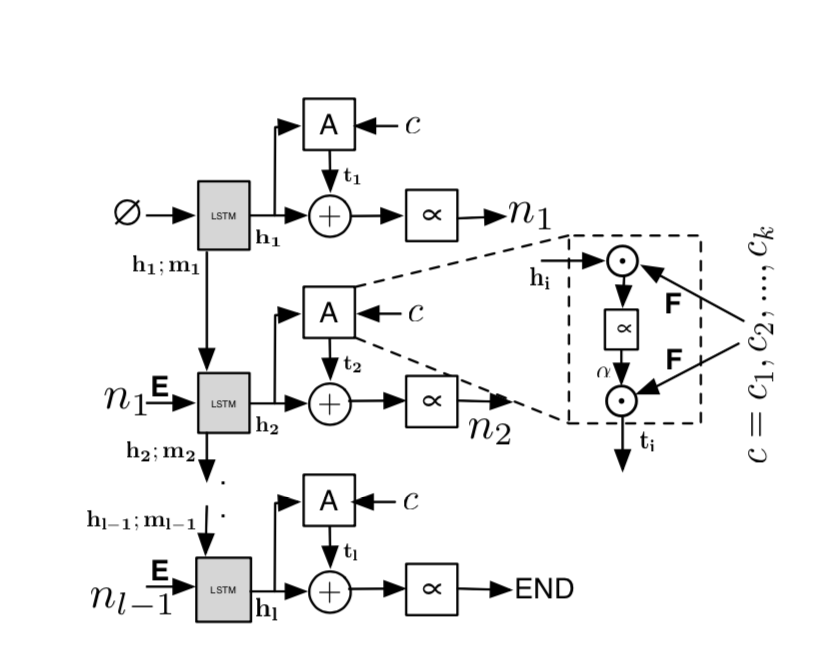
\includegraphics[width=0.5\linewidth]{ModelPics/Iyer_etal.png}
    \caption{Iyer et als Code NN, taken from \cite{iyer_summarizing_2016}}
    \label{fig:Iyer}
\end{figure}

\cite{loyola_neural_2017}




%  %drew inspiration from successes in recurrent neural networks in language modelling (CITE), and
% used of a neural attention model over source code tokens, combined with an LSTM accepting sequences of natural language tokens, to give distributions over the next token in the sequence.
% Specifically they modelled the probability of generating a length $l$
% descriptive sequence as a product of conditional probabilities the previous $l-1$ tokens
% % word sequence as a product of conditional probabilities over the next word, derived from the attentions and hidden states of the LSTM.
% % 
% $$P(\{n\}) = \prod_{i=1}^lp(n_i | n_1, ..., n_{i-1} ) $$

% where each conditional distribution was proportional to the combinations of the attentional representation and hidden state of the LSTM at that time.

% $$$$

% where 
% over the next word, whether the probabilities 

%  a distributional representation (PARA) of the source code would be calculated by an attention mechanism \cite{luong_effective_2015}, before being combined in addition with the hidden state $h_i$ of an LSTM (cite shmidthuber) and passed through a softmax layer to chose the next word in the description sequence. Each sequence 

 Summaries of Code changes - 


% Hindle's work  


% They built on work by Hindle, supported by SU
% This work ignores semantic information that could be benefitial. 

% This work specifically occurs at the level fo programming comments,

% A number of other pieces of work have since worked higher level summaries of code.
% Sridhara etc al templates
% Code NN summarization
% Related to semantic parsing - inverted. 
% Summaries of Code changes - 

% At the other end of the spectrum, code naming is treated a extremem summarization task, and has seen development.
% Other related tasks ro such include variable naming.

All